\documentclass[]{standalone}

\usepackage{adjustbox}

\usepackage{amsmath}

\usepackage{mathrsfs}

\usepackage{circuitikz}
\usepackage{tikz}
\usetikzlibrary{arrows, patterns, decorations.pathmorphing, backgrounds, positioning, fit, petri, shapes, trees, matrix, chains, decorations, decorations.pathreplacing, decorations.fractals, calc,snakes,trees, decorations.markings}

\usepackage{color}
\definecolor{soton}{RGB}{7,51,71}
\colorlet{comms}{red!50!yellow}
\colorlet{payld}{pink!50!purple}
\colorlet{obdh}{green!50!black}

\begin{document}

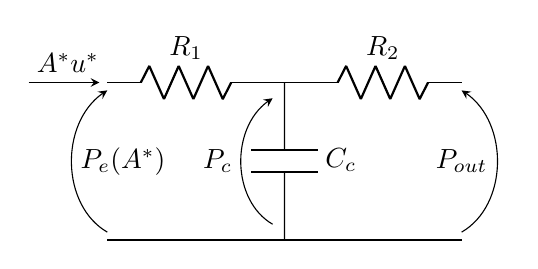
\begin{tikzpicture}

\draw (0,0) to[R=$R_1$] (2,0) -- (2.5,0) to[R=$R_2$] (4.5,0);
\draw (2.25,0) to[C=$C_c$] (2.25,-2);
\draw (0,-2) -- (4.5,-2);
\draw[-stealth] (2.1,-1.8) to [out=150,in=210] (2.1,-0.2);
\node at (1.4,-1) {$P_c$};

\draw[-stealth] (0,-1.9) to [out=150,in=210] (0,-0.1);
\node at (0.2,-1) {$P_e(A^*)$};

\draw[-stealth] (4.5,-1.9) to [out=30,in=-30] (4.5,-0.1);
\node at (4.5,-1) {$P_{out}$};

\draw[-stealth] (-1,0) -- (-0.1,0);
\node[above] at (-0.5,0) {$A^* u^*$};

\end{tikzpicture}


\end{document}